En esta sección esperamos poder brindar una breve introducción a los temas que son relevantes para el desarrollo y la implmentación de este proyecto. La dividiremos en tres partes: qué dataset elegimos y por qué; brindaremos una breve explicación que busca proveer al lector de las herramientas para poder interpretar la implementación; finalmente, explicaremos porque la aplicación de SIMD resulta pertinente a este problema.

\subsection{El dataset: MNIST}

El dataset MNIST\footnote{\url{http://yann.lecun.com/exdb/mnist/}} está compuesto por imágenes de dígitos manuscritos del 0 al 9, con una resolución de $28\times 28$ píxeles. A su vez, ya viene dividido en un training set de 60000 ejemplos (en particular, nosotros solo usamos 50000), y un test set de 10000.

Es un dataset que, por su simplicidad, está pensado para ser usado como un primer benchmark rápido para modelos, pudiendo abstraerse de las complicaciones inherentes al preprocesamiento de datos. 

En vista de que el objetivo central que se persigue es el de conseguir una optimización desde el punto de vista del tiempo de ejecución de las operaciones básicas, y no de la precisión del modelo (es decir, no nos interesa una red particularmente compleja), encontramos que este dataset se ajusta bien a nuestras necesidades: es lo bastante chico como para poder manejarlo con el hardware del que disponemos, pero no tanto como para no permitirnos hacer un análisis interesante. Un dataset más complicado no nos aportaría nada.

\subsection{Redes Neuronales Artificiales}

Daremos una explicación muy acotada al \emph{scope} de este trabajo, de en qué consiste una Red Neuronal Artificial (RN).

Una RN es uno de los tantos modelos encuadrados dentro del paradigma del aprendizaje supervisado\footnote{\url{https://en.wikipedia.org/wiki/Supervised_learning}}. El elemento fundamental de las redes neuronales son las \emph{neuronas}. Una neurona computa una función con múltiples inputs y un output (todos números reales). La imagen (\ref{fig:neurona}) ilustra la estructura general de una neurona.

La función que ejecuta la neurona tiene dos partes. Primero una lineal (también llamada \emph{transfer function}), en la cual se multiplica a cada uno de los inputs $x_i$ por un cierto peso $w_i$, y posteriormente se los suma. En la suma suele participar un término independiente, $b$. Es decir,

$$z = \sum w_i x_i + b$$

Luego, se le aplica a $z$ la llamada \emph{función de activación}, que nos dará el output de la neurona. Dicho función puede ser cualquiera que vaya de los reales a los reales, aunque típicamente se escojen ciertas funciones no lineales (se puede probar fácilmente que usar una función lineal no agrega mayor capacidad para aproximar funciones). En particular, para este trabajo usaremos como función de activación la función sigmoidea definida como sigue:

$$\sigma(z) = \frac{1}{1 + e^{-z}}$$

\begin{figure}
  \begin{center}  
    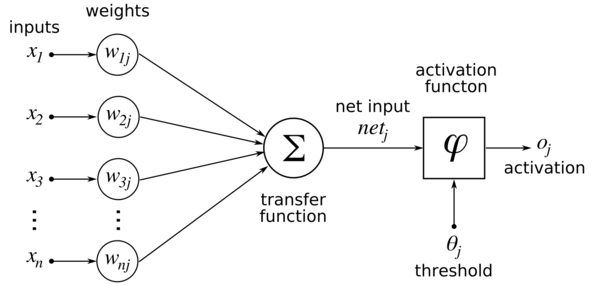
\includegraphics[width=0.7\linewidth]{imgs/neuron.png}
  \end{center}
  \caption{Estructura general de una neurona}
  \label{fig:neurona}
\end{figure}

En general, una red neuronal va a consistir de muchas neuronas interconectadas (es decir que el output de una se vuelve el input de otra). Esto puede hacerse con diversas arquitecturas. En particular, nosotros usamos una de las más básicas que es la de Feedforward Neural Network. Esta es una arquitectura por capas o layers (donde cada capa es un conjunto de neuronas que no están interconectadas entre sí), en la cual el output de cada neurona de una capa alimenta al input de todas las neuronas de la capa siguiente (\emph{full connected}). En la siguiente imagen se ilustra esta arquitectura

\begin{figure}[H]
  \begin{center}  
    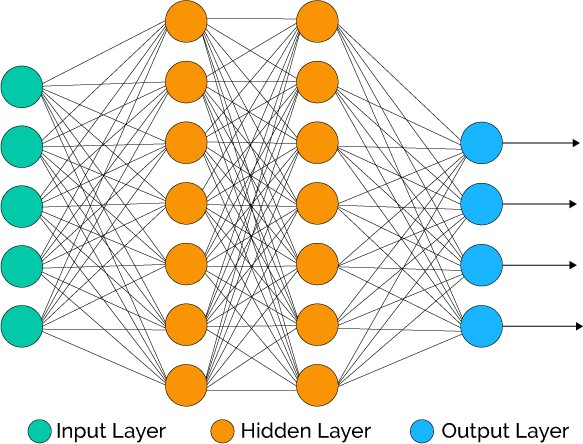
\includegraphics[width=0.7\linewidth]{imgs/multilayer_net.jpg}
  \end{center}
  \caption{Estructura general de una feedforward neural network}
  \label{fig:general_net}
\end{figure}

Puede verse que se diferencian tres tipos de capas: input layers, hidden layers y output layers. La primera y la última son bastante autoexplicativas; las capas ocultas (hidden) reciben ese nombre por el hecho de que los cómputos que realizan no son visibles por el usuario de la red, en contraposición con los inputs y los outputs que sí son ``visibles''. A una red como la de la imagen se la llama 3-layer neural network (no se cuenta la capa de input).

Pasemos ahora a la parte más importante, que es el algoritmo de entrenamiento de la red. Ante todo es importante entender que lo que queremos aprender son los parámetros $w_{ij}$ y $b_i$. Además, es necesario definir una función de costo: es decir, una función que nos indique cuan ``lejos'' están las predicciones de las etiquetas verdaderas. Luego, el objetivo del entrenamiento será seleccionar los parámetros $w_{ij}$ y $b_i$ que minimizen esta función.

Usaremos como función de costo el Error Cuadrático Medio (ECM)

$$C(w, b) = \frac{1}{2n}\sum_{x}{||y(x) - a||^2}$$

donde $w$ y $b$ son todos los parámetros de nuestra red, $y(x)$ es el output de la red para el input x, $a$ es el target verdadero para el input $x$, y $n$ es la cantidad de casos de entrenamiento.

La heurística de optimización usada es la versión más simple de Gradient Descent, por lo que en cada epoch ajustaremos los parámetros de la siguiente forma:

$$w_{ij} := w_{ij} - \eta \frac{\partial C}{\partial w_{ij}}$$
$$b_i := b_i - \eta \frac{\partial C}{\partial b_i}$$

donde $\eta$ es el \emph{learning rate} que determina cuanto queremos modificar nuestros parámetros en una iteración, y $\frac{\partial C}{\partial v}$ es la derivada parcial de $C$ respecto del parámetro $v$.

La pregunta que queda entonces es cómo calculamos las derivadas parciales. Para esto se utiliza un algoritmo conocido como \emph{backpropagation}. Recibe este nombre en contraposición al \emph{forwardpropagation}, que es la pasada que se realiza sobre la red para calcular el output. Es decir que ahora querremos atravesar la red en sentido opuesto para calcular las derivadas parciales.
